\cm{Intro spiel}

\section{Molecule theory}
\label{theory:molecules}

\cm{
  \begin{itemize}
      \item Summary of basic energy structure: e-, vib, rot
      \item Making a MOT
      \item Microwave state selection
      \item Magnetic trapping
  \end{itemize}
}

\section{Chip trap theory}
\label{theory:chips}

% TODO Motivate chip traps in introduction
% TODO Set up with discussion of QP and IP traps including equations for their
% fields
In this section I will describe how a magnetic trap can be formed using
currents on the surface of a chip.

\subsection{Simple wire traps}

We begin our discussion by considering a simple case of a one-dimensional trap.
This will be formed of a straight wire, which we approximate to have infinite
length, and an external bias field. The magnetic field due to the wire is
described by the Biot-Savart law~\cite{}, having magnitude
%
\begin{equation}
  B = \frac{\mu_0 I}{2 \pi r}
\end{equation}
%
where $I$ is the current in the wire and $r$ is the distance from it. The
direction of the field obeys the \cm{right} hand rule. When the bias field
$\mathbf{\tilde{B}}$ is
homogenous and uniform across all space, there will be a point when the two
fields cancel. Taking the wire to run along the $y$ axis, and the bias field to
point in the $x$ direction, there will be a field zero at
%
\begin{equation}
  z = \frac{\mu_0 I}{2 \pi \tilde{B}}
  \label{theory:eqn:height}
\end{equation}
%
as is shown in \cm{a figure}. The field close to the zero approximates a
\cm{2D?} quadrupole field with gradient
%
\cm{TODO.}
%
The trapping frequency \cm{in directions..?}

\begin{figure}
  \centering
  \begin{subfigure}[b]{0.45\textwidth}
    \centering
    \hfill{}
    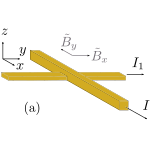
\includegraphics[width=0.8\textwidth]{figs/theory/wires/dimple_150.pdf}
    \hfill{}
  \end{subfigure}
  \begin{subfigure}[b]{0.45\textwidth}
    \centering
    \import{figs/theory/wires}{simpleheat_alone.pgf}
  \end{subfigure} \\
  \begin{subfigure}[b]{0.45\textwidth}
    \centering
    \import{figs/theory/wires}{simpleheat_y.pgf}
  \end{subfigure}
  \begin{subfigure}[b]{0.45\textwidth}
    \centering
    \import{figs/theory/wires}{simpleheat_z.pgf}
  \end{subfigure}
  \caption{\cm{TODO: change this dimple thing to a simple wire cartoon}}
\end{figure}


%\begin{figure}
%  \centering
%  \import{figs/theory/wires}{simpleheat.pgf}
%  \caption{}
%  \label{TBD}
%\end{figure}

\cm{Are there more bias fields to consider?}

Such a trap is of course only two-dimensional, since there is no confinement
along the axis of the wire. However it is simple to introduce confinement in
this direction -- introduce a second wire perpendicular to the first. When this
second wire has a current much lower than the original $I_2 \ll I$, we can
treat its contribution to the field as a perturbation. \cm{Somethign about sign
  of $I_2$ is important.} Such a configuration is
known as a dimple trap, and produces a field \cm{TODO equations}.

\cm{NOTE: IP trap, (or QP with more bias?)}

\begin{figure}[htb]
    \centering
    \begin{tabular}[t]{cc}
\begin{subfigure}{0.3\textwidth}
    \centering
    \smallskip
    \includegraphics[width=\textwidth]{figs/theory/wires/dimple.pdf}
\end{subfigure}
    &
        \begin{tabular}{c}% if you add [t], than sub images are pushed down
        \smallskip
            \begin{subfigure}[t]{0.4\textwidth}
                \centering
                  \import{figs/theory/wires}{dimpleheat_alone.pgf}
            \end{subfigure}\\
            \begin{subfigure}[t]{0.4\textwidth}
                \centering
                  \import{figs/theory/wires}{dimple_x.pgf}
            \end{subfigure}
        \end{tabular}\\
    \end{tabular}
  \caption{HELP!}
\end{figure}

% TODO introudce $h$ as trap height
Consider the case where the sign of $I_2$ is reversed, now we have a maximum in
the magnetic field at height $h$. This might not seeem to be of any use, but
combining two such anti-traps can create a local minium in which weak-field
seekers can be trapped. This configuration is called the H-trap, and is
shown in \cm{ref fig}. Such a trap can be configured as a quadrupole (when the
currents in the off-axis wires are parallel) or as a Ioffe-Pritchard (when the
currents in the off-axis wires are anti-parallel). In the former case we can
think of the field zero being formed due to the cancellation of the
contribution from the off-axis wires. In the latter case, the off-axis wires
produce fields in the same direction, and so the trap centre is non-zero.

\begin{figure}
  \centering
  \begin{subfigure}[b]{0.4\textwidth}
    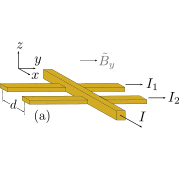
\includegraphics[width=\textwidth]{figs/theory/wires/Htrap.pdf}
    %\vspace{0.1mm}
  \end{subfigure}
  \begin{subfigure}[b]{0.4\textwidth}
    \import{figs/theory/wires}{Hx.pgf}
  \end{subfigure}
  \caption{}
  \label{TBD}
\end{figure}

Although the H-trap provides a clear method of creating a three dimensional
microtrap, it is not always convenient to have to use three distinct wires.
Fortunately the H-trap can be approximated by a single wire, either in a
U-shape for the quadrupole variant, or a Z-shape for the Ioffe-Pritchard
variant. These are pictured in \cm{figure}.



\cm{
  \begin{itemize}
      \item Basic idea of 2D traps
      \item How close can we get to surface? %(Blackbody, note from Charles in interview? (about charge??))
      \item Extend to 3D
      \item U and Z, majorana losses
      \item dimple traps
      \item Typical trap freqs (for small traps, used in sideband cooling)
  \end{itemize}
  }

\section{Quantum optics}
\label{theory:QO}

In this section we introduce a general model of molecules interacting with
light.  Since this is a broad field, I will focus the discussion only on the
details that are directly used in this thesis.  Namely the calculation of the
scattering rates for molecules in a light field and the coupling of molecules
to a light field in a resonator.

%\cm{Do I also need to discuss the normal mw spectroscopy in free space?}

\subsection{Scattering rates}

\cm{To come later}

\subsection{Cavity quantum electrodynamics}

A key part of the motivation for a molecule chip trap is the idea that
integrated microwave guides can be used to couple photons to the rotational
transitions of the molecules. Of particular interest is the idea
that a resonator can be used to perform this coupling, leading to the
ability to perform sideband-cooling to the motional ground state, state readout
and coupling between individually-trapped molecules~\cite{Andre2006}. This is
similar to techniques used in atom chips~\cite{Treutlein2008} and for optical
resonators coupling to atomic energy levels~\cite{SchleierSmith2011}.
% TODO Better cite in this last bit?

For our purposes, the coupling of a single molecule and the microwave field can
be treated as the coupling of a two-level system to a quantum mode of a cavity
field. The canonical description of such a system is given by the familiar
Jaynes-Cummings Hamiltonian (JCH) in the rotating wave
approximation~\cite{gerry_knight_2004}
%
\begin{equation}
  H_\text{JC} = \hbar\omega_c a^\dagger a + \frac{\hbar \omega_0}{2} \sigma_z +
  \frac{\hbar\Omega}{2}(a^\dagger \sigma_- + a\sigma_+)
  \label{theory:eqn:JCH}
\end{equation}
%
where $a$ ($a^\dagger$) is the annihilation (creation) operator of the photons,
$\Omega$ is the Rabi frequency of the interaction, $\sigma_i$ with $i\in{x, y,
z}$ are the Pauli matrices, and $\sigma_\pm =
(\sigma_x \pm i\sigma_y)/2$ are the raising and lowering operators of the
molecule state. The
detuning of the cavity resonance from that of the spin is $\Delta = \omega_0 -
\omega_c$. The system is shown in \mysubfigref{theory:fig:JCHstates}{a}.

\begin{figure}
  %\includegraphics{}
  \cm{Part (a) is image of JCH system, (b) is state manifold without coupling
  or detuning, (c) is state manifold with coupling (d) adds detuning (similar
  to Bohi fig 1)}
  \caption{\cm{TODO}}
  \label{theory:fig:JCHstates}
\end{figure}

We denote the ground (exicted) state of the molecule as $\ket{g}$ ($\ket{e}$).
The light field state can be taken to be a Fock state ($\ket{n}$ with $n \in
\mathbb{Z}$). Note that the final term in equation~\ref{theory:eqn:JCH}) has
the effect of exciting the ground state while absorbing a photon
($\ket{g}\ket{n} \leftrightarrow \ket{e}\ket{n-1}$) or lowering the excited state
and releasing a photon ($\ket{e}\ket{n} \leftrightarrow \ket{g}\ket{n+1}$).

Following the procedure in \inlineref{gerry_knight_2004}, we can see that this
mixing of the states results in a shift of the energy levels to create the
dressed states
%
\begin{align}
  \ket{+, n} &= \cos\Phi_n \ket{g}\ket{n} + \sin\Phi_n \ket{e}\ket{n+1} \\
  \ket{-, n} &= -\sin\Phi_n \ket{g}\ket{n} + \cos\Phi_n \ket{e}\ket{n+1}
\end{align}
%
with
%
\begin{equation}
  \tan(2\Phi_n) = \frac{\Omega\sqrt{n+1}}{\Delta}
\end{equation}
%
and having shifted energies
%
\begin{equation}
  E_{\pm, n} = (n+1)\hbar\omega_c \pm \frac{\hbar}{2}\sqrt{\Omega^2(n+1) +
  \Delta^2}.
  \label{theory:eqn:JCHenergies}
\end{equation}
%
It is useful to consider the manifold of states as depicted in
\myfigref{theory:fig:JCHstates}.  
%TODO This fig
Note that in the limit of no coupling
($\Omega = 0$) and no detuning ($\Delta = 0$) the energies are that of the bare
states, and $\ket{g}\ket{n+1}$ is degenerate with $\ket{e}\ket{n}$, as in part
(b) of the subfigure. Introducing coupling ($\Omega \neq 0$) lifts this
degeneracy, as in part (c). When the detuning is non-zero ($\Delta \neq 0$)
there is additional offset due to the second term in
\myeqref{theory:eqn:JCHenergies}, see part (d) of the figure.

The strong coupling r\'egime is reached when the coupling $g=2\Omega$ is
greater than the rate of decay from the cavity $\kappa = \omega_0 / Q$, where
$Q$ is called the quality factor of the cavity. The coupling parameter is
related to the transition dipole moment $d$ and the amplitude of the electric
field $E_0$ by
%
\begin{equation}
  \hbar g = \frac{d E_0}{2}.
\end{equation}
%
For the resonator, the amplitude of the electric field can be expressed in
terms of the cavity parameters by considering the electric field density
%
\begin{equation}
  \frac{1}{2} \epsilon_0 E_0 = \frac{\hbar \omega_0}{V}
\end{equation}
%
where $V$ is the volume of the mode in the cavity. The idea is to confine the
molecules in a trap that is on the $w=\SI{10}{\micro\meter}$ scale (see
chapter~\ref{overview}) and the resonator will necessarily have a length on the
scale of $\lambda_0 = 2\pi c / \omega_0$, therefore $V\approx w^2\lambda_0$.
Hence we have that
%
\begin{equation}
  g = \sqrt{\frac{2\pi c d^2}{\hbar \epsilon_0 w^2 \lambda_0^2}}.
\end{equation}

% TODO maybe move this whole sentence above
For the rotational \CaF{} transitions that we introduced above, in
section~\ref{theory:molecules} $d = \mu/\sqrt{3}$ with $\mu =
\SI{31}{\debye}$.
%
The coupling strength is therefore expected to be
%
% See nbs/2022-02-08_coupling.nb
\begin{equation}
  \frac{g}{2\pi} = \SI{20}{\kilo\hertz}
\end{equation}
%
and for strong coupling a cavity quality of
%
\begin{equation}
  Q = \frac{\omega_0}{g} > 1.7 \times 10^5
\end{equation}
%
is required.
